% !Mode:: "TeX:UTF-8"
% The first line is for editors like, WinEdt, to specify the encoding
\documentclass[a4paper,11pt]{article}
\usepackage[a4paper,vmargin=1in,hmargin=1.5in]{geometry}

\usepackage[
    colorlinks,linkcolor=blue,anchorcolor=blue,citecolor=green,
    pdfauthor={Susen Zhao <zhaosusen@gmail.com>}, pdftitle={LaTeX入门教程: 介绍}
    ]{hyperref}

\usepackage{fontspec,xltxtra,xunicode}
\usepackage{xeCJK}
\defaultfontfeatures{Mapping=tex-text}
% set Chinese fonts
\setCJKmainfont[BoldFont={Adobe 黑体 Std},ItalicFont={Adobe 楷体 Std}]{Adobe 宋体 Std}
\setCJKsansfont{Adobe 黑体 Std}
\setCJKmonofont{Adobe 仿宋 Std}
% set western fonts
\setmainfont{Adobe Garamond Pro}

\usepackage{listings}
\usepackage{xcolor}
\usepackage{graphicx}
\usepackage{subfig}
\usepackage{fancyhdr}
\usepackage{caption}
\usepackage{amsmath}

\newcommand{\cmd}[1]{~\texttt{#1}~}

\setlength{\parindent}{22pt}
\linespread{1.25}\selectfont

\DeclareCaptionLabelFormat{figcaption}{\textbf{图}~#2~}
\captionsetup[figure]{labelformat=figcaption,labelsep=space}

\title{用\LaTeX{}写漂亮的实验报告}
\author{\textsc{Susen Zhao}\\
\href{mailto:zhaosusen@gmail.com}{\small\texttt{zhaosusen@gmail.com}}}
\date{}

\begin{document}

\maketitle
\tableofcontents

% !Mode:: "TeX:UTF-8"
% The first line is for editors like, WinEdt, to specify the encoding

\section{前言}
我接触\LaTeX{}大概有一年了,从开始的一个absolute beginner到现在,也算是初窥门径,基本能用\LaTeX{}来写日常的实验报告、数学建模论文
乃至毕业论文,从了解文档的基本结构到现在也能写一点文类和宏包(虽然只是一丁点),在这些过程中,我深刻地体会到了\LaTeX{}的高效、稳定
以及高质量,这是Microsoft Word之类的字处理软件(word processor)
所难以企及的高度\footnote{对于一般的需求来说,Word也可以达到可接受的质量,但一定要学会使用样式。}。

因为自己用着觉得不错,我就很想把\LaTeX{}推广给更多的同学使用。目前看来,\LaTeX{}在中国有一定的使用群体,但是仍然很小众,真正欣赏她的人
更是少之又少。在\LaTeX{}在科技排版界已经成为事实标准的今天,
国内的诸多高校以及科技出版机构仍然抗拒使用\LaTeX{},许多老师更是指明要求使用Word排版,我觉得这是一件很可怕的事情。暂不说Word的排版质量,
首先它是一个昂贵的商业软件,虽然针对高校学生有优惠,但是既然有免费并且更先进,几乎可以称为state of the art的\TeX{}系列,我们为什么要花钱
去赞助evil的Microsoft呢?当然,我知道更多的同学还在使用盗版的Office软件,那更应该把他们解放出来了。

说到这里,许多同学可能要问,“\LaTeX{}容易学吗?”“我并不是学工科的,也能用\LaTeX{}吗?”。我在这里想说的是,如果你是计算机科学、数学、物理
及相关专业的,我极力推荐你使用\LaTeX{};如果你是Art类专业的,比如英语专业,需要使用西文完成论文的,我也非常推荐你使用\LaTeX{}——因为\TeX{}
的西文排版引擎是非常先进的,大型专业排版软件如InDesign、PageMaker等也只能勉强与其比肩。

说了这么多,\LaTeX{}与Word这类字处理软件到底有什么本质的区别或优点呢?网上这类对比非常多,就我个人而言,感受到的主要有以下几点:
\begin{enumerate}

\item Word的传统文件格式是私有的、封闭的二进制文件\footnote{自Word 2003起开放了文档格式,为使用zip压缩的一组XML文件,但是也非常复杂,难以解析。},
容易损坏(就不用我问有多少同学的文档被Word弄坏过吧);
而\LaTeX{}的源文件则是是字节码,不容易损坏,并且有很高的可移植性,几乎可以在任何平台打开、编辑,并且可以方便地输出为PDF格式。

\item 相比于Word这一类字处理软件,\LaTeX{}拥有更好的输出效果。在\TeX{}排版引擎内部有极佳的断字以及断行算法,以求达到最佳的美感(仅对于英文来说);
并且,\TeX{}内部对长度的定义非常精细,精细到你无法想象,从而可以对文本进行精确地定位,完成高质量的输出。

\item \LaTeX{}的思想是内容与结构分离,只要预定义好了文档结构,写作者就可以主要关注文档的内容,而不需要边写作还要边考虑文档的格式,比如字体大小、
样式等等与内容无关的内容;而Word虽然是一种“所见即所得”的工具,但是对于格式的实时关注对于写作来说是一个distraction,会分散写作者的注意力。

\item \LaTeX{}对于写作长文档,尤其是科技论文有很大的优势。使用\LaTeX{},章节编号、图形编号、表格编号、参考文献等等都可以自动生成,并且可以方便地
实现交叉引用;而在Word里,类似的功能不仅操作复杂,有时候还要借助第三方的、同样是收费的插件。

\item \LaTeX{}对于数学公式的排版是公认的最好,没有之一。只需要简单地对比一下Word和\LaTeX{}生成的公式效果就可以发现。

\end{enumerate}

除了这些优点,下面我还想针对计算机专业的同学说几句,那就是用\LaTeX{}能更好地与计算机\textbf{交流}。在没有计算机排版的年代,作者要
在自己的底稿上注明文章的结构,由排字工进行排版;而\LaTeX{}继承了这一优良的传统。\LaTeX{}是一个强大的宏(macro)语言,在文档结构上也可以称为
标记语言,常见的标记语言有HTML,XML等。所谓标记语言也就是用一定的标记标明文档的结构,比如你要告诉\LaTeX{}某行字是文章的标题,或者某行字是
一节的小标题,那么应该怎么做呢?Okay,就是像这样:
\begin{quote}
\begin{verbatim}
\title{这是文章标题}
\section{这是节标题}
\subsection{这是小节标题}
\end{verbatim}
\end{quote}
这里,用~\verb+\somecommand{}+~标明文档的结构。

那么,我们再来看一下,在Word里,一般的同学会怎么做:输入一行字,比如“实验目的”,然后选中,
设置为宋体,三号字,加粗,无缩进;如果有新的标题,比如“实验结果”,那么重复一遍上面的过程,或者使用格式刷。嗯,看起来还不错,也许对于鼠标
操作快的同学,甚至还比输入一个标记来得快捷。但是,考虑这样的情况,对于一个长文档,比如毕业论文,某一天老师突然让你把所有的标题改成黑体,那对于
像刚才那样Word操作习惯的同学,必须一个个地改格式;如果老师还希望标题可以编号,那就更惨了。

对于\LaTeX{},这些都可以通过简单的设置来搞定,因为
事先已经用标记把文章的结构标好了,只需要对指定的结构使用指定的格式,就可以一次性地把问题解决;并且,\LaTeX{}可以自动为章节编号,并且可以按你
指定的格式来编号。当然,Word也有样式功能和大纲模式,这与\LaTeX{}的工作方式类似,但是据我了解,没有合适的引导,大部分同学是不会用样式和大纲模式的,
并且,Word也没有直观地提示你使用。况且,用符号(或语言)与计算机交流的效率和准确性远远高于使用鼠标指点。(所以,计算机系的同学们,动手coding吧,不要
怕写程序,要学会真正与计算机交流的方式。)

总而言之,在我看来,对于计算机专业的同学来说,\LaTeX{}是再合适不过的一个文档准备软件了,更不必提她是基于\TeX{}的,而\TeX{}是计算机科学界的巨擘
Prof.~Donald E. Knuth的大作。同时,\LaTeX{}也是向大部分科技类国际期刊、会议投稿的第一选择;如果你用心,也照样可以用\LaTeX{}作出优美的艺术品,
当然,\TeX{}本身就是一件艺术品。

% !Mode:: "TeX:UTF-8"
% The first line is for editors like, WinEdt, to specify the encoding

\section{快速入门}
在这一节里,我将根据自己的使用经验,写一个\LaTeX{}的快速入门,让同学们能在较短的时间里开始使用\LaTeX{}。
\subsection{基本概念}
本文中可能出现一些术语,在这里事先解释一下。
\begin{description}
\item[\TeX] \TeX{}是由Prof.~Donald E. Knuth创造的一套排版系统,最初的目的是为了排版他的巨著《计算机程序设计艺术》
(\emph{The Art of Computer Programming})第二卷。在第一版出版的时候,使用的还是活字排版,但到第二版付印之时,
出版本书的Addison-Wesley出版社已经换用了计算机排版系统,Knuth教授发现新的排版系统把他的巨作排得很差,他一怒之下,
决定自己写一个排版系统,也就成就了后来的\TeX{}。\TeX{}源于希腊字母$\tau\epsilon\chi$,在希腊语中是科学和艺术的意思。
\TeX{}提供了若干底层排版命令,是一套强大的宏语言,可以在其上定义更高层的排版命令。为了方便使用,Knuth自己编写了
一套宏,称为Plain \TeX{},但还是不够方便,于是有了后来的\LaTeX{}。

\item[\LaTeX] \LaTeX{}是Leslie Lamport在\TeX{}之上编写的一组宏包(package),目的是将内容和格式分离,并且根据科技论文的
排版需求,提供了很多环境,如列表、定义、证明等。\LaTeX{}还提供了方便的交叉引用机制,为文章的写作提供了很大的方便。
目前\LaTeX{}的最新版本是~\LaTeXe{}。

\item[文类] 文类是定义文档类型的文件,是使用\TeX{}和\LaTeX{}命令编写的,其扩展名为\cmd{.cls},其作用是提供某种
文档样式的规范,比如页边距、行距、字体和字号、标题格式等许多定义文档样式的参数。

\item[命令] \LaTeX{}源文件是用文本和命令编写而成的,命令是用来告诉\LaTeX{}应该执行怎样的排版操作。\LaTeX{}的命令
都是由反斜杠符号\cmd{\textbackslash}加上一串英文字母构成的,字母区分大小写。

\item[宏包] 由于\TeX{}是一种宏语言,从而可以通过宏定义扩展其功能,存储这些宏的文件就称为宏包,其扩展名为\cmd{.sty}。
许多强大的功能都是使用前人编写的宏包来完成的。

\item[衬线体] 衬线体(serif)是有衬线的字体,衬线就是字脚的装饰部分,
英文中的衬线体如图~\ref{fig:enserif}~所示\footnote{图像来源:\url{http://en.wikipedia.org/wiki/Serif}},
从上到下依次是无衬线体、衬线体以及衬线用红色标出的衬线体;
中文中的衬线体如图~\ref{fig:zhserif}~所示,从左到右依次是衬线用红色标出的衬线体、衬线体以及无衬线体。
据说,衬线来源于上古时代的书法家使用树枝或石块在泥土上写字所留下的字脚装饰。
衬线体一般用于正文,其可读性较强,并且被认为比较正统。

\item[无衬线体] 无衬线体(Sans-serif)是没有衬线的字体,英文中的无衬线体如图~\ref{fig:enserif}~所示,其中最上面的字体为无衬线体;
中文中的无衬线体如图~\ref{fig:zhserif}~所示,最右边的字体为无衬线体。无衬线体一般用于标题或标志牌。

\begin{figure}[!h]
\centering
\subfloat[英文的衬线体与无衬线体]{
  \label{fig:enserif}
  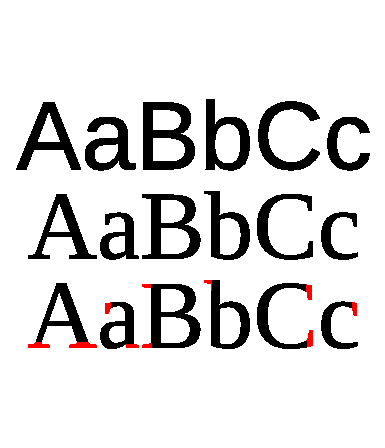
\includegraphics[width=0.4\textwidth]{figures/Eng_serif.eps}
}
\hspace{0.1\textwidth}
\subfloat[中文的衬线体与无衬线体]{
  \label{fig:zhserif}
  
\includegraphics[width=0.4\textwidth]{figures/Chinese_serif.eps}
}
\caption{衬线体与无衬线体}
\label{fig:serif}
\end{figure}

\item[等宽字体] 等宽字体(monospaced font)是指每个字符宽度相同的字体,与之相对的是每个字符宽度不尽相同的字体,
称为比例字体(proportional font),
如图~\ref{fig:promono}~所示\footnote{图像来源:\url{http://zh.wikipedia.org/wiki/File:Propvsmono.svg}},
上面的是比例字体(Minion Pro),下面的是等宽字体(Courier)。
一般来说,比例字体的可读性较强,但是早期由于技术限制,打字机或计算机使用的为等宽字体。
目前等宽字体使用较多的场合是用于显示程序代码。

\begin{figure}[!h]
\centering
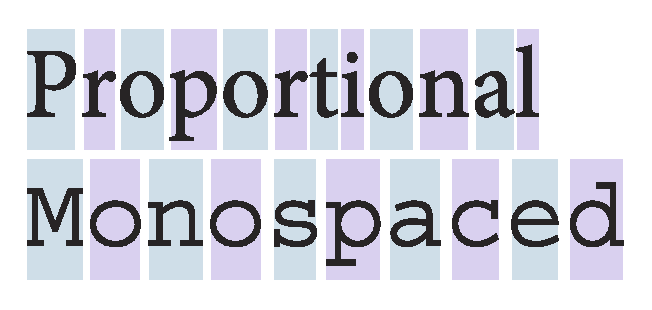
\includegraphics[width=0.6\textwidth]{figures/monospace.eps}
\caption{比例字体与等宽字体}
\label{fig:promono}
\end{figure}

\end{description}

\subsection{文档结构}
本节主要介绍\LaTeX{}的文档结构。基本的文档结构如下:
\begin{quote}
\begin{verbatim}
\documentclass[文类选项]{文类}
\usepackage[宏包选项]{宏包}
% 导言区
\begin{document}
% 正文区
\end{document}
\end{verbatim}
\end{quote}

\subsection{特殊符号}

\subsection{插图}

\subsection{交叉引用}

\subsection{中文的处理} 

\end{document}
